%% PX1 manuscript, Elsevier CAS single-column template (cas-sc), as used by the group's earlier submission.
%% Target: ISPRS Journal of Photogrammetry and Remote Sensing (first submission may be any format, "Your Paper Your Way").
%% Revised draft, Nov 2026.

\documentclass[a4paper,fleqn]{cas-sc}

\usepackage[numbers,sort&compress]{natbib}
\usepackage{booktabs}
\usepackage{multirow}
\usepackage{amsmath,amssymb}
\usepackage{xcolor}
\usepackage{siunitx}
\sisetup{detect-all}

\begin{document}
\let\WriteBookmarks\relax
\def\floatpagepagefraction{1}
\def\textpagefraction{.001}
\let\printorcid\relax

\shorttitle{Physics-checked test-time adaptation for SAR flood mapping}
\shortauthors{M.S. Hasan et al.}

\title [mode = title]{Physics-checked test-time adaptation for SAR flood mapping with flood-level miss-rate calibration}

\author[1]{MD Sakib Hasan}
\author[1]{Mostofa Seum}
\author[1]{Meer Mursalin}
\author[1]{Tanvir Ahmed}[]
\cormark[1]
\ead{tanvir.ahmed@aiub.edu}
\author[1]{Rifath Mahmud}
\author[1]{Syeda Anika Tasnim}

\affiliation[1]{organization={Department of Computer Science, American International University-Bangladesh (AIUB)},
            addressline={408/1, Kuratoli, Khilkhet},
            city={Dhaka},
            postcode={1229},
            country={Bangladesh}}

\cortext[1]{Corresponding author}

\begin{abstract}
Deep networks that map floods in Sentinel-1 radar images lose accuracy on floods unlike their training data, and an emergency leaves no labels to retrain them. Test-time adaptation updates a model on the unlabelled images of a new flood but can also degrade it, and a threshold of 0.5 does not control how much water a map misses. We study both together. The adaptation re-estimates batch-normalisation statistics, then self-trains on pseudo-labels checked against radar and terrain physics (dark, low-lying, flat pixels). The threshold is calibrated on other, labelled floods with flood events as the unit, so that the mean miss rate stays below a target. Models trained on Sen1Floods11 were tested on 26 Kuro Siwo events and, in a pre-registered test, on 30 MMFlood activations. On Kuro Siwo at a 20\% miss-rate target the method reached 0.677 intersection over union (IoU), against 0.565 without adaptation and 0.457--0.574 for six adaptation baselines including TENT, EATA, SAR and CoTTA, none of which beat the unadapted model once miss rates were matched; it was level with supervised fine-tuning on labelled Kuro Siwo floods (0.657). With the threshold calibrated on Sen1Floods11 alone, unadapted models missed 58\% of the water; after the proposed adaptation, 6\%. On MMFlood the method beat TENT and batch-norm adaptation at a matched miss rate (28 of 30 floods) but not the unadapted model, source-only calibration failed, and IoU stayed near 0.2 because much labelled water there is not dark. Adaptation methods should be compared at matched miss rates.
\end{abstract}

%% Highlights are uploaded as a separate file (highlights.txt), as Elsevier asks.


\begin{keywords}
flood mapping \sep synthetic aperture radar \sep test-time adaptation \sep conformal prediction \sep height above nearest drainage \sep Sentinel-1
\end{keywords}

\maketitle
\hypersetup{pdftitle={Physics-checked test-time adaptation for SAR flood mapping with flood-level miss-rate calibration},pdfauthor={MD Sakib Hasan, Mostofa Seum, Meer Mursalin, Tanvir Ahmed, Rifath Mahmud, Syeda Anika Tasnim}}

%% =====================================================================
\section{Introduction}
\label{sec:intro}

Floods affect more people than any other natural hazard, and the share of the world's population living in flood-exposed areas is rising \citep{tellman2021exposure}. Synthetic aperture radar (SAR) sees through clouds and at night, which makes Sentinel-1 \citep{torres2012sentinel1} the main source of rapid flood maps: open water reflects little radar energy back to the sensor and appears dark. Operational systems such as the Copernicus Global Flood Monitoring service combine thresholding, change detection and terrain masks \citep{salamon2021gfm,twele2016s1chain,zhao2021exclusion}, and deep networks trained on labelled benchmarks \citep{bonafilia2020sen1floods11,bountos2024kurosiwo,montello2022mmflood} now outperform thresholds on images like those they were trained on \citep{bentivoglio2022review,helleis2022benchmark}.

Two problems limit their use in an emergency. First, accuracy drops sharply on floods unlike the training data: different landscapes, seasons, radar calibration and labelling conventions \citep{bentivoglio2022review,turkmenli2025dgflood}. In our experiments, models trained on Sen1Floods11 missed 81\% of the water in Kuro Siwo at the default threshold. Labels for the new flood are not available in time to retrain. Test-time adaptation (TTA) updates a model on the unlabelled images it is asked to map, for example by re-estimating batch-normalisation statistics \citep{li2018adabn,schneider2020covariate}, minimising prediction entropy \citep{wang2021tent} or self-training on its own confident predictions \citep{tarvainen2017meanteacher,wang2022cotta}. \citet{chen2026cimttda} recently showed that pseudo-label self-training improves SAR inundation maps across coastal flood events. TTA can also fail, however: a model can confirm and amplify its own mistakes \citep{niu2022eata,niu2023sar}, and nothing in the unlabelled images reveals when this happens.

Second, a flood map is usually produced by thresholding a probability at 0.5, and nothing tells the user how much flooding the map misses. For emergency response, missed flood water is the costlier error. Deep networks are poorly calibrated \citep{guo2017calibration}, and calibration degrades further on new data. Heuristic uncertainty estimates exist for flood maps \citep{gal2016dropout,lakshminarayanan2017ensembles,chen2026uncertaintyflood}, but they do not bound an error rate. Conformal prediction gives distribution-free guarantees \citep{vovk2022alrw,angelopoulos2023gentle}, and conformal risk control can bound the expected false negative rate of a segmentation \citep{angelopoulos2024crc}. For flood maps it has been used to build pixel-level prediction sets on optical images \citep{konidakis2025cpflood} and, for SAR, to meet a user-set risk level and abstain outside the training distribution \citep{li2026crcflood}. These studies calibrate and test within one data distribution. Whether a calibrated threshold survives the move to a new dataset, and what adaptation does to it, has not been examined.

This paper studies the two together. Our hypothesis is that SAR flood physics, namely that open water is dark and lies low in flat terrain, provides an independent check on the pseudo-labels a model produces for itself, and that adaptation and calibration have to be evaluated jointly: a method that looks best at threshold 0.5 need not be best once every method is held to the same miss rate. The contributions are:
\begin{itemize}
\item A label-free test-time adaptation for SAR flood mapping that re-estimates batch-normalisation statistics and then self-trains on pseudo-labels corrected by a per-flood radar threshold, height above nearest drainage (HAND) \citep{renno2008hand,nobre2011hand} and slope. Relative to the teacher--student self-training of \citet{chen2026cimttda}, the new element is the physics check and its combination with batch-norm re-estimation.
\item Flood-level calibration of the map threshold with flood events as the unit: a mean rule from conformal risk control, and a per-flood rule under which a chosen share of floods meets the miss-rate target. Both apply existing theory; the contribution is the unit, the per-flood statement and the test of both under dataset shift.
\item An evaluation at matched miss rates on three datasets with events as the statistical unit, against six adaptation baselines on Kuro Siwo (TENT and AdaBN on all three datasets) and a supervised fine-tuning reference, including a pre-registered test on 30 MMFlood activations that were not used for any design decision \citep{nosek2018prereg}, and a test of calibration without any label from the target dataset.
\item Three findings. (i) Rankings change once the miss rate is matched: on Kuro Siwo, TENT, EATA, SAR, CoTTA and AdaBN all look strong at 0.5, and none of them beats the unadapted model at a calibrated threshold, while the proposed method does by 0.11 IoU and is level with supervised fine-tuning. (ii) On Kuro Siwo, adaptation is what makes a threshold calibrated on the source floods valid: without it the maps miss 58\% of the water against a 20\% target, with the proposed method 6\%, with 25 of 26 events below the target. (iii) On MMFlood the proposed method beats TENT and AdaBN at a matched miss rate but not the unadapted model, source-only calibration fails, and absolute accuracy is too low for use; we report why.
\end{itemize}

Section~\ref{sec:related} reviews related work, Section~\ref{sec:method} describes the method, Section~\ref{sec:setup} the data and experimental protocol, Section~\ref{sec:results} the results, and Section~\ref{sec:discussion} discusses them with their limitations.

%% =====================================================================
\section{Related work}
\label{sec:related}

\subsection{SAR flood mapping}
Classical SAR flood mapping thresholds backscatter, often per tile or with parametric fits \citep{otsu1979threshold,martinis2009nrt,chini2017hsbt}, uses change detection against a pre-flood image \citep{giustarini2013change,clement2018multitemporal}, and refines the result with terrain and context \citep{twele2016s1chain,landuyt2019assessment}. Probabilistic variants estimate per-pixel flood probabilities \citep{giustarini2016probabilistic,krullikowski2023gfmensemble}. Known failure modes are flooded vegetation and urban areas, where water is bright rather than dark \citep{tsyganskaya2018vegetation,zhao2024urbansarfloods}. Deep learning has become standard since public benchmarks appeared \citep{bonafilia2020sen1floods11,mateogarcia2021worldfloods,drakonakis2022ombrianet,bountos2024kurosiwo,montello2022mmflood}, with convolutional networks \citep{nemni2020unosat,bai2021basnet,konapala2021s1s2}, change-detection networks applied globally \citep{misra2025globalfloods} and geospatial foundation models, which are mostly pretrained on optical imagery and use transformer encoders without batch normalisation \citep{jakubik2023prithvi}. Reviews identify generalisation to new floods and uncertainty as the main open problems \citep{bentivoglio2022review,lee2025geoaiflood}.

\subsection{Terrain priors}
HAND, the height of a pixel above the nearest drainage channel \citep{renno2008hand,nobre2011hand}, is widely used to rule out implausible flooding. It serves as a post-hoc mask or exclusion layer \citep{twele2016s1chain,zhao2021exclusion,misra2025globalfloods}, as a prior in Bayesian flood mapping \citep{tupas2023handprior}, as a network input \citep{tian2026deepsar} and in rule-based refinement \citep{hansen2025ribe}. Elevation can also shape the training loss \citep{sami2024evanet}. More broadly, physics-guided machine learning uses scientific knowledge to constrain data-driven models \citep{karpatne2017tgds,reichstein2019deep,willard2022integrating}. We use terrain and radar physics at a different point: to correct pseudo-labels during label-free adaptation on the target flood.

\subsection{Domain adaptation and test-time adaptation}
Domain shift is a long-standing problem in remote sensing \citep{tuia2016darsreview}. Unsupervised domain adaptation with self-training \citep{lee2013pseudolabel,zou2018cbst,hoyer2022daformer} needs the source data during adaptation. TTA adapts with target data only: AdaBN re-estimates batch-normalisation statistics \citep{li2018adabn,schneider2020covariate}, TENT minimises entropy \citep{wang2021tent}, teacher-student methods use pseudo-labels from an exponential-moving-average teacher \citep{tarvainen2017meanteacher,wang2022cotta}, and reliability filtering aims to avoid collapse \citep{niu2022eata,niu2023sar}; see \citet{liang2025ttasurvey} for a survey. TTA has been applied to remote-sensing segmentation and classification \citep{wang2024rsselfprompt,liang2024lscdtta} and to SAR coastal inundation \citep{chen2026cimttda}. For floods, label-efficient alternatives include adversarial adaptation with label refinement \citep{akiva2021h2onet}, semi-supervised pseudo-labelling \citep{paul2021semisup}, cross-modal distillation \citep{garg2023crossmodal}, unsupervised change detection on time series \citep{yadav2022unsupts} and domain generalisation across events \citep{turkmenli2025dgflood}. The closest work is CIM-TTDA \citep{chen2026cimttda}, which adapts a SAR water-segmentation model to each new coastal flood with pseudo-labels and an exponential-moving-average teacher; our self-training stage follows the same recipe. None of these methods checks pseudo-labels against physics, and none is evaluated at a controlled miss rate.

\subsection{Conformal prediction and risk control}
Conformal prediction produces distribution-free guarantees under exchangeability \citep{vovk2022alrw,lei2018distfree,angelopoulos2023gentle}. Risk-controlling prediction sets \citep{bates2021rcps}, conformal risk control \citep{angelopoulos2024crc} and learn-then-test \citep{angelopoulos2021ltt} extend it to general losses such as the false negative rate of a segmentation \citep{mossina2024conformalseg}. Under distribution shift the guarantee needs weighting or degrades gracefully \citep{tibshirani2019covshift,barber2023beyond}; when data come in groups, the groups rather than their members must be exchangeable \citep{dunn2023hierarchical}. In flood mapping, \citet{konidakis2025cpflood} produced pixel-level prediction sets for optical images, and \citet{li2026crcflood} combined a density-aware network with conformal risk control so that SAR flood maps meet a user-set risk level, with abstention outside the training distribution and set-valued predictions. Our use of conformal risk control is therefore not new in itself. What differs is that flood events are the calibration unit, that a per-flood statement is added to the mean one, and that we measure what happens to both when the calibration floods come from a different dataset than the flood being mapped, with and without test-time adaptation.

%% =====================================================================
\section{Method}
\label{sec:method}
Fig.~\ref{fig:method} summarises the three steps applied to each new flood event.

\begin{figure}[t]
\centering
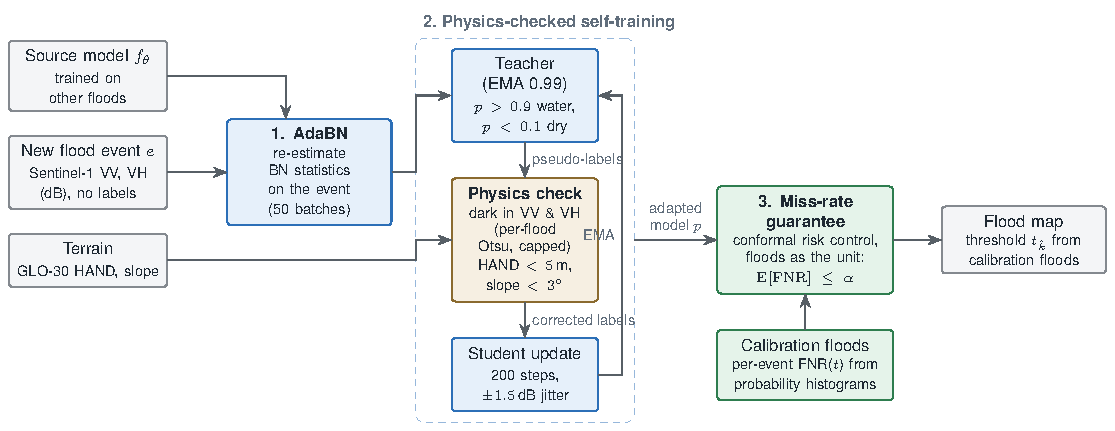
\includegraphics[width=\textwidth]{figures/fig_method.pdf}
\caption{Overview of the method. (1) AdaBN re-estimates batch-normalisation statistics on the unlabelled event. (2) A mean teacher produces confident pseudo-labels, which are corrected with a per-flood radar darkness test and HAND/slope limits before each student update. (3) The decision threshold is calibrated on other, labelled flood events so that the miss rate averaged over floods (mean rule) or the miss rate of at least a share $1-\delta$ of floods (per-flood rule) stays below $\alpha$.}
\label{fig:method}
\end{figure}

\subsection{Problem setting}
A segmentation network $f_\theta$ is trained on labelled Sentinel-1 chips (VV and VH backscatter in dB) from a set of source floods. At test time it receives the chips $\mathcal{X}_e$ of a new flood event $e$, without labels, and must output a binary flood map. For each pixel $f_\theta$ gives a water probability $p$; the map is $\{p \ge t\}$ for a threshold $t$. We want (i) maps that are as accurate as possible on $e$ and (ii) a threshold that keeps the miss rate (false negative rate, FNR) at a level $\alpha$ chosen by the user. Adaptation uses no labels at all. Calibrating the threshold needs labelled floods, but none from the target flood; Section~\ref{sec:calib} states which floods can serve and Section~\ref{sec:results} tests what happens when they come from another dataset.

\subsection{Batch-normalisation re-estimation}
Radar calibration and land cover differ between datasets, which shifts the statistics of intermediate features. Following AdaBN \citep{li2018adabn}, we reset the running mean and variance of every batch-normalisation layer and re-estimate them as a cumulative average over 50 batches of eight random $256\times256$ crops (with random rotations and flips) of the event's chips. No weights are trained; this takes about 10\,s per event.

\subsection{Physics-checked self-training}
After AdaBN, a copy of the network serves as teacher and the network itself as student. For 200 steps, a batch of eight random crops is drawn from the event. The teacher's water probability $p$ gives a pseudo-label of water where $p>0.9$, dry where $p<0.1$, and no label otherwise. These pseudo-labels are then checked against physics:
\begin{itemize}
\item \textbf{Per-flood dark threshold.} For each polarisation, an Otsu threshold \citep{otsu1979threshold} is computed on the backscatter of all chips of the event, together with the mean $\mu_d$ of the darker class. The dark threshold is the midpoint between them, capped at $-15$\,dB (VV) and $-22$\,dB (VH) so that a flood with little open water cannot turn dry land into water. The rule was fixed before any of the reported runs.
\item \textbf{Low and flat terrain.} HAND below 5\,m, taken from the global 30\,m HAND dataset derived from the Copernicus GLO-30 DEM \citep{glo30hand2022}, and slope below $3^\circ$ from the DEM.
\item \textbf{Correction.} Pixels that are dark in both polarisations, low and flat are labelled water if the teacher's probability is at least 0.1; if the teacher is confident they are dry ($p<0.1$), the conflict is left unlabelled.
\end{itemize}
The student is trained on the corrected pseudo-labels with class-weighted cross-entropy (weights 1 and 3 for dry and water) and Adam (learning rate $10^{-4}$), with a random backscatter offset of up to $\pm1.5$\,dB and Gaussian noise added to its input. The teacher follows the student as an exponential moving average (decay 0.99), as in mean-teacher self-training \citep{tarvainen2017meanteacher,chen2026cimttda}. The teacher is used for the final map. Without the physics check, the procedure is plain self-training.

\subsection{Flood-level miss-rate calibration}
\label{sec:calib}
For each method we store, per event, the histogram of predicted water probabilities (1000 bins) separately for water and dry pixels. This gives, for every threshold $t_k=k/1000$, the event's miss rate $\mathrm{FNR}_e(t_k)$. Flood events, not pixels, are the unit of calibration \citep{dunn2023hierarchical}: pixels within a flood are strongly dependent, whereas floods can plausibly be treated as exchangeable draws when they come from the same population. We use two rules, both computed from $n$ labelled calibration floods.

\paragraph{Mean rule.} Following conformal risk control \citep{angelopoulos2024crc}, the threshold is
\begin{equation}
\hat{k}_{\mathrm{mean}} = \max\Big\{k : \frac{n}{n+1}\,\frac{1}{n}\sum_{i=1}^{n}\mathrm{FNR}_i(t_k) + \frac{1}{n+1} \le \alpha\Big\}.
\label{eq:mean}
\end{equation}
Because FNR is bounded by 1 and does not increase as the threshold falls, $\mathbb{E}[\mathrm{FNR}_{n+1}(t_{\hat{k}})]\le\alpha$ when the calibration floods and the new flood are exchangeable. This bounds the miss rate averaged over floods. It says nothing about a single flood, and individual floods can miss far more than $\alpha$.

\paragraph{Per-flood rule.} To make a statement about each flood, let $k_i=\max\{k:\mathrm{FNR}_i(t_k)\le\alpha\}$ be the highest threshold at which calibration flood $i$ still meets the target. The threshold is the $\lfloor\delta(n+1)\rfloor$-th smallest of $k_1,\dots,k_n$ (and $0$, mapping everything as water, if $\lfloor\delta(n+1)\rfloor=0$). By the standard split-conformal argument \citep{vovk2022alrw,lei2018distfree}, a new exchangeable flood then meets the target with probability at least $1-\delta$:
\begin{equation}
\mathbb{P}\big[\mathrm{FNR}_{n+1}(t_{\hat{k}_{\mathrm{flood}}})\le\alpha\big]\ \ge\ 1-\delta .
\label{eq:flood}
\end{equation}
We report $\alpha=0.2$ with $\delta=0.2$ (at least four floods in five miss at most 20\% of their water) and $\delta=0.1$. The price is a lower threshold and therefore more false alarms than under the mean rule.

\paragraph{Where the calibration floods come from.} Both statements hold only if the calibration floods are exchangeable with the new one. We evaluate two settings. In \emph{same-dataset} calibration each event is calibrated on all other events of its dataset (leave one flood out); this uses labels of other floods from the target dataset and is the favourable case. In \emph{source-only} calibration the thresholds are computed once, on the 11 Sen1Floods11 floods, and applied unchanged to another dataset, so that no label of the target dataset is used at any point. Exchangeability is then not assured \citep{tibshirani2019covshift,barber2023beyond}, and whether the target is met becomes an empirical question that depends on how comparable the model's scores are across datasets.

%% =====================================================================
\section{Data and experimental setup}
\label{sec:setup}

\subsection{Datasets}
Table~\ref{tab:data} summarises the data. All three datasets provide Sentinel-1 VV and VH backscatter with expert flood labels.
\begin{itemize}
\item \textbf{Sen1Floods11} \citep{bonafilia2020sen1floods11}: 446 hand-labelled $512\times512$ chips from 11 flood events. Models were trained on the standard training split (252 chips) and selected on its validation split.
\item \textbf{Kuro Siwo} \citep{bountos2024kurosiwo}: the published dataset covers 43 flood events and stores its labelled Sentinel-1 GRD patches ($224\times224$ pixels at 10\,m, each with a pre-flood image) as shards of more than 0.5\,TB in total. We did not download all of it. We read a short window every 512\,MB of every shard of the training and test splits and kept the first six complete patches in each window, about one patch in 50, spread evenly through each event. The sample holds 1,962 patches from 33 events; the 26 events with at least eight patches were evaluated. By default permanent water and flood water both count as water, as in Sen1Floods11; we also report scores with permanent water ignored, which is the MMFlood convention.
\item \textbf{MMFlood} \citep{montello2022mmflood}: 95 Copernicus EMS activations in 333 region folders. Activations overlapping Kuro Siwo (within 300\,km and 365 days) or Sen1Floods11 (within 300\,km and the same or adjacent year) were excluded (144 folders). Images were resampled from 20\,m to 10\,m and cut into $512\times512$ chips with at least 50\% valid radar, at most 48 per folder; OpenStreetMap permanent water that the EMS mask labels dry was ignored. The 69 folders with at least eight chips (1,240 chips) come from 30 activations in 21 countries.
\end{itemize}
HAND was resampled from the GLO-30 HAND tiles \citep{glo30hand2022} onto every chip grid. Fig.~\ref{fig:sites} shows where the events are.

\begin{figure}[t]
\centering
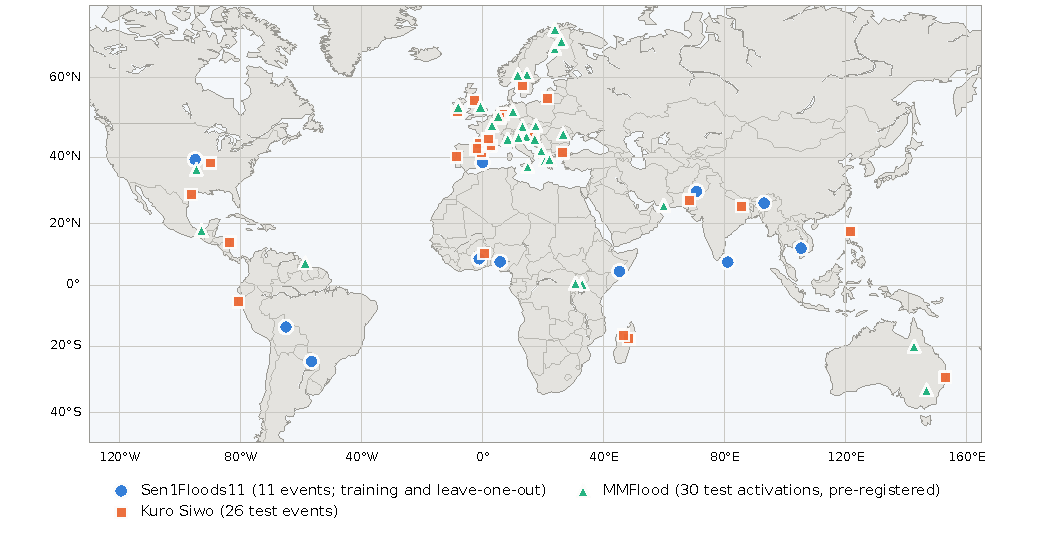
\includegraphics[width=\textwidth]{figures/fig_sites.pdf}
\caption{Locations of the Sen1Floods11 events (centroid of each event's footprint), the 26 Kuro Siwo test events and the 30 MMFlood test activations (activation centre from the MMFlood metadata).}
\label{fig:sites}
\end{figure}

\begin{table}[t]
\caption{Datasets and their role. Events are the statistical unit for every test and for calibration.}
\label{tab:data}
\centering
\begin{tabular}{llll}
\toprule
Dataset & Events & Chips & Role \\
\midrule
Sen1Floods11 & 11 & 446 & training; leave-one-flood-out test; source-only calibration \\
Kuro Siwo & 26 (of 33 sampled) & 1,962 & cross-dataset test; development of the method \\
MMFlood & 30 activations (69 folders) & 1,240 & pre-registered final test \\
\bottomrule
\end{tabular}
\end{table}

\subsection{Models and training}
The main model is a five-level U-Net \citep{ronneberger2015unet} with batch normalisation \citep{ioffe2015bn} and 32 base channels, trained from scratch on VV and VH (normalised with Sen1Floods11 training statistics) for 60 epochs on random $256\times256$ crops with flips and rotations, AdamW \citep{loshchilov2019adamw} (learning rate $10^{-3}$, weight decay $10^{-4}$, cosine schedule) and class-weighted cross-entropy. Three models were trained with different seeds; on the standard Sen1Floods11 test split they reach a water-class IoU of $0.660\pm0.005$ (pixels pooled over the split). For the leave-one-flood-out test on Sen1Floods11, one model per held-out flood was trained on the other floods. A second backbone, a U-Net with an ImageNet-pretrained \citep{deng2009imagenet} ResNet-34 encoder \citep{he2016resnet,iakubovskii2019smp}, was trained with the same recipe (learning rate $3\times10^{-4}$, three seeds). A variant of it was trained on Sen1Floods11 plus the Kuro Siwo sample, drawing equal numbers of chips from each per epoch.

\subsection{Compared methods}
\label{sec:compared}
All adaptation methods start from the same models and use the same crops, batch size and number of steps (200).
\begin{itemize}
\item \textbf{No adaptation}, and \textbf{AdaBN} alone \citep{li2018adabn}.
\item \textbf{Entropy minimisation on batch-norm weights}: TENT \citep{wang2021tent} (Adam, learning rate $10^{-3}$); EATA \citep{niu2022eata}, which uses only reliable pixels (entropy below $0.4\ln 2$), re-weights them and anchors the weights with a Fisher penalty (estimated here with the unadapted model on the first 20 target batches); and SAR \citep{niu2023sar}, which adds sharpness-aware updates ($\rho=0.05$) to the reliable-pixel loss.
\item \textbf{Teacher--student self-training}: plain self-training with an exponential-moving-average teacher, following \citet{chen2026cimttda}; and CoTTA \citep{wang2022cotta}, which averages the teacher over augmentations (flips and backscatter offsets), trains all weights on the soft teacher output and restores 1\% of the weights to their source values at every step.
\item \textbf{Physics-checked self-training}, without AdaBN and after AdaBN, with either fixed thresholds ($-18$\,dB VV, $-25$\,dB VH, relative height and slope) or the adaptive rule of Section~\ref{sec:method}. AdaBN followed by the adaptive rule is the proposed method.
\item \textbf{Model-free references}: an Otsu threshold on VV \citep{otsu1979threshold}, and on Kuro Siwo a change-detection rule that uses the pre-flood image: a pixel is flood water if it is dark after the flood (below the per-flood dark threshold) and its VV dropped by more than the Otsu threshold of the difference image, capped at $-3$\,dB \citep{giustarini2013change,clement2018multitemporal}.
\item \textbf{Supervised reference}: same-dataset calibration uses labelled floods of the target dataset, so we also ask what those labels buy when used for training. The Kuro Siwo events were split into five folds by event; each source model was fine-tuned on the labelled chips of four folds (1,500 steps, Adam, learning rate $10^{-4}$) and tested on the events of the fifth. The recipe was fixed in advance and not tuned.
\end{itemize}
TENT and AdaBN were run on all three datasets. EATA, SAR, CoTTA and the supervised reference were added in revision and run on Kuro Siwo only; plain self-training was run on Sen1Floods11 and Kuro Siwo. Kuro Siwo distinguishes permanent water from flood water. The main scores count both as water, as Sen1Floods11 does; a second set of scores ignores permanent-water pixels (``flood water only'').

\subsection{Metrics and statistics}
For each event and method we report IoU of the water class at threshold 0.5 and at the calibrated thresholds (mean rule at $\alpha=0.1, 0.2, 0.3$; per-flood rule at $\alpha=0.2$ with $\delta=0.2$ and $0.1$), the mean and the worst per-event miss rate, the number of events that meet the target, precision, and the false-alarm rate (the share of dry pixels mapped as water). Comparing methods at a calibrated threshold compares them at a matched miss rate, which a fixed threshold of 0.5 does not. Values are averaged over the three models per event. The pre-registered hypotheses on MMFlood were tested with one-sided Wilcoxon signed-rank tests over activations \citep{wilcoxon1945,demsar2006} and Holm correction \citep{holm1979}. All other comparisons are post hoc; they use two-sided Wilcoxon tests with Holm correction within each table and are labelled as such.

\subsection{Protocol and pre-registration}
The physics check, its thresholds and the combination with AdaBN were developed on Sen1Floods11 and Kuro Siwo; Kuro Siwo therefore served as a development set. Before any MMFlood data were downloaded, we wrote down the primary method (chosen by a fixed rule from the Kuro Siwo results), the preprocessing and exclusion rules, and four hypotheses: under the mean rule at the 20\% target with same-dataset calibration, the primary method beats TENT (H1) and AdaBN (H2); it beats no adaptation at threshold 0.5 (H3); and the mean miss rate at the 20\% target is at or below 0.20 (H4). After download, and before any result was seen, we fixed the activation (rather than the region folder) as the statistical unit. The text was written in a dated working document, which is included with the code; it was not deposited in a public registry before the test, so its date cannot be verified by a third party. Everything else was added after the MMFlood results were known and is exploratory: the second backbone, the EATA, SAR and CoTTA baselines, the per-flood rule, source-only calibration, the fine-tuning reference and the flood-water-only scores.

%% =====================================================================
\section{Results}
\label{sec:results}

\subsection{Sen1Floods11, leave one flood out}
On held-out Sen1Floods11 floods, the in-domain setting, all methods except TENT lie within 0.03 IoU of each other (Table~\ref{tab:s1f}), and no difference between the proposed method and no adaptation or AdaBN is significant with 11 floods. TENT is the weakest at every threshold. With only 10 calibration floods the mean rule is conservative: at the 20\% target the realised mean miss rate is 0.12--0.13, and IoU drops by about 0.07 relative to threshold 0.5. Targets below $1/(n+1)\approx0.09$ cannot be met with an informative threshold, because the correction term alone exceeds them (Fig.~\ref{fig:guarantee}a, d).

\begin{table}[t]
\caption{Sen1Floods11, leave one flood out (11 floods, radar only): mean IoU at threshold 0.5, under the mean rule (Eq.~\ref{eq:mean}) and under the per-flood rule (Eq.~\ref{eq:flood}), with the number of floods that meet the 20\% target under the per-flood rule. Best value per column in bold.}
\label{tab:s1f}
\centering
\small
\begin{tabular}{lcccccc}
\toprule
 & & \multicolumn{3}{c}{Mean rule, target $\alpha$} & \multicolumn{2}{c}{Per-flood rule, $\alpha=\delta=0.2$} \\
\cmidrule(lr){3-5}\cmidrule(lr){6-7}
Method & 0.5 & 10\% & 20\% & 30\% & IoU & Floods meeting \\
\midrule
No adaptation & 0.551 & 0.189 & 0.479 & 0.543 & \textbf{0.475} & 9.0/11 \\
Self-training \citep{chen2026cimttda} & 0.550 & 0.193 & 0.486 & 0.551 & 0.461 & 9.0/11 \\
TENT & 0.504 & 0.168 & 0.442 & 0.527 & 0.405 & 9.0/11 \\
AdaBN & 0.573 & 0.182 & 0.479 & 0.562 & 0.459 & 9.0/11 \\
Physics-checked self-training, fixed rule & 0.566 & 0.193 & 0.491 & 0.565 & 0.465 & 9.0/11 \\
Physics-checked self-training, adaptive rule & 0.556 & 0.150 & \textbf{0.497} & 0.551 & 0.463 & 9.0/11 \\
AdaBN + physics check, fixed rule & \textbf{0.575} & \textbf{0.195} & 0.481 & \textbf{0.571} & 0.439 & 9.0/11 \\
AdaBN + physics check, adaptive rule (proposed) & 0.561 & 0.171 & 0.494 & 0.557 & 0.459 & 9.0/11 \\
\bottomrule
\end{tabular}

\end{table}

\subsection{Kuro Siwo}
The domain gap is large (Table~\ref{tab:ks}): without adaptation the models miss 81\% of the water at threshold 0.5 (IoU 0.186). Same-dataset calibration alone recovers much of the gap (0.565 at the 20\% target), because the threshold moves to where the new dataset needs it; this gain comes from labels of other Kuro Siwo floods and not from adaptation. The fair comparison between adaptation methods is therefore at a calibrated threshold, where all of them realise the same mean miss rate (0.17 at the 20\% target, Fig.~\ref{fig:guarantee}e). There, none of the six baselines improves on the unadapted model. AdaBN, EATA, SAR and CoTTA are level with it (0.558--0.574 against 0.565; no difference is significant), and plain self-training and TENT are worse (0.457 and 0.467). At threshold 0.5, by contrast, TENT, EATA, SAR, CoTTA and AdaBN all look strong (0.563--0.598 against 0.186): what they gain at 0.5 is the operating point that calibration provides anyway. The proposed method is better than every baseline at the matched miss rate (0.677; $+0.112$ over no adaptation, better on 23 of 26 events, Holm-corrected $p=2\times10^{-4}$; $+0.115$ over AdaBN, 23 of 26, $p=2\times10^{-4}$; $+0.119$ over EATA, 23 of 26, $p=2\times10^{-4}$; $+0.113$ over SAR, 21 of 26, $p=5\times10^{-4}$; $+0.103$ over CoTTA, 21 of 26, $p=5\times10^{-4}$; $+0.209$ over TENT, 25 of 26, $p=3\times10^{-6}$; post hoc tests, Holm over the 16 comparisons made at this target). Its advantage is largest at strict targets (0.565 at the 10\% target against 0.456 without adaptation and 0.327--0.436 for the baselines).

\paragraph{Supervised reference.} Fine-tuning the source models on the labelled chips of other Kuro Siwo events reaches 0.661 IoU at threshold 0.5 and 0.657 at the 20\% target. The proposed method, which uses no Kuro Siwo label for adaptation, is level with it (0.677; better on 11 of 26 events, $p=0.71$), and its miss rates are more even: under the mean rule its worst event misses 38\% of the water, against 64\% for the fine-tuned models. Fine-tuning is ahead at the strictest target (0.592 against 0.565 at 10\%). The fine-tuning recipe was not tuned, so this is a reference point and not an upper bound on what target labels can give.

\begin{table}[t]
\caption{Kuro Siwo, 26 unseen events, U-Net trained on Sen1Floods11, radar only, same-dataset calibration (mean over three models): mean IoU at threshold 0.5, under the mean rule and under the per-flood rule, with the number of floods that meet the 20\% target under the per-flood rule. Best value per column among the label-free methods in bold; the fine-tuned models use labels of other Kuro Siwo events.}
\label{tab:ks}
\centering
\small
\begin{tabular}{lcccccc}
\toprule
 & & \multicolumn{3}{c}{Mean rule, target $\alpha$} & \multicolumn{2}{c}{Per-flood rule, $\alpha=\delta=0.2$} \\
\cmidrule(lr){3-5}\cmidrule(lr){6-7}
Method & 0.5 & 10\% & 20\% & 30\% & IoU & Floods meeting \\
\midrule
No adaptation & 0.186 & 0.456 & 0.565 & 0.550 & 0.529 & 21.7/26 \\
Self-training \citep{chen2026cimttda} & 0.174 & 0.360 & 0.457 & 0.490 & 0.432 & 21.3/26 \\
TENT & 0.576 & 0.327 & 0.468 & 0.576 & 0.413 & 21.3/26 \\
AdaBN & 0.570 & 0.400 & 0.562 & 0.584 & 0.535 & 21.0/26 \\
Physics-checked self-training, adaptive rule & 0.627 & 0.500 & 0.666 & \textbf{0.655} & 0.577 & 21.0/26 \\
AdaBN + physics check, fixed rule & 0.669 & 0.525 & 0.664 & 0.649 & 0.625 & 21.0/26 \\
AdaBN + physics check, adaptive rule (proposed) & \textbf{0.673} & \textbf{0.565} & \textbf{0.677} & 0.644 & \textbf{0.652} & 21.0/26 \\
\midrule
Otsu threshold on VV (no model) & 0.456 & -- & -- & -- & -- & -- \\
\bottomrule
\end{tabular}

\end{table}

\paragraph{What each part contributes.} Physics-checked self-training without AdaBN reaches almost the same IoU as the full method under the mean rule (0.666 against 0.677; $p=0.71$). AdaBN matters elsewhere: at threshold 0.5 (0.627 against 0.673), for the worst flood (the method without AdaBN misses up to 85\% of the water on one event, the full method at most 38\%; Table~\ref{tab:transfer}), under the per-flood rule (0.577 against 0.652; better on 24 of 26 events, $p=6\times10^{-6}$) and, most of all, when no target labels are available for calibration (Section~\ref{sec:transfer}). The two parts therefore do different jobs: the physics check recovers water the model misses, and re-estimating the batch-norm statistics makes the scores comparable from flood to flood and from dataset to dataset, which is what a shared threshold needs.

Fig.~\ref{fig:guarantee} shows the whole trade-off for the mean rule. For every target between 0.05 and 0.5 the realised mean miss rate stays just below the target on all three datasets and for every method (panels d--f), so the methods differ only in how much accuracy they keep.

\begin{figure}[t]
\centering
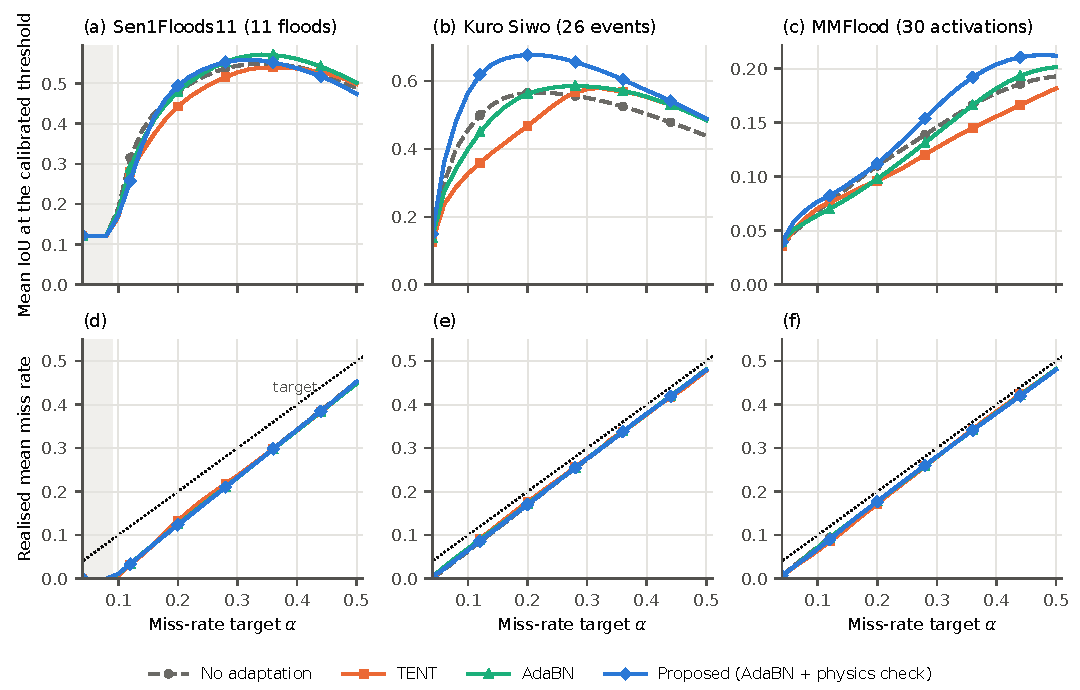
\includegraphics[width=\textwidth]{figures/fig_guarantee.pdf}
\caption{Accuracy and validity of the mean rule with same-dataset calibration as the miss-rate target $\alpha$ varies. (a--c) Mean IoU at the calibrated threshold; (d--f) realised mean miss rate, with the target as a dotted line. Sen1Floods11: 11 floods, leave one flood out; Kuro Siwo: 26 events; MMFlood: 30 activations; mean over three models for the last two. Shading: targets below $1/(n+1)$ cannot be met with an informative threshold.}
\label{fig:guarantee}
\end{figure}

Per event (Fig.~\ref{fig:ksevents}), the mean hides a wide spread: at the 20\% target, between 16 and 20 of the 26 events meet the target under the mean rule, depending on the method. The baselines occasionally fail badly: on their worst event AdaBN, EATA and SAR miss 85--88\% of the water, TENT 92\% and CoTTA 74\%. The worst event of the proposed method misses 38\%.

\begin{figure}[t]
\centering
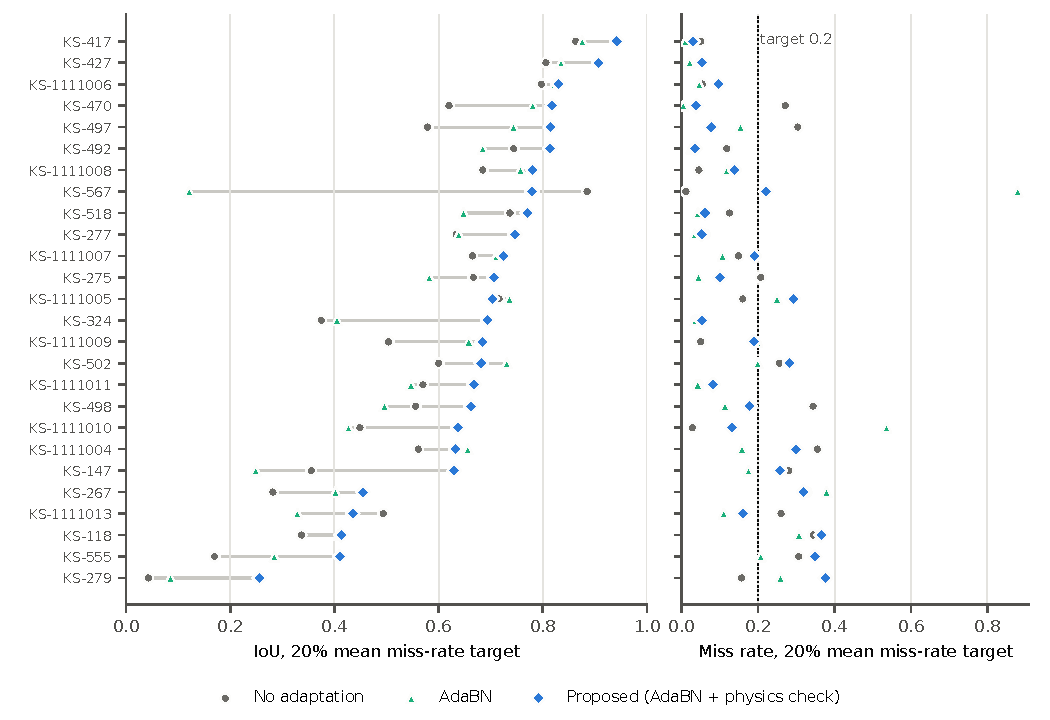
\includegraphics[width=\textwidth]{figures/fig_ks_events.pdf}
\caption{Kuro Siwo, per event, mean rule at the 20\% target with same-dataset calibration (mean over three models): IoU (left) and miss rate (right) without adaptation, with AdaBN, and with the proposed method. Events are sorted by the IoU of the proposed method.}
\label{fig:ksevents}
\end{figure}

The physics check also produces cleaner maps (Table~\ref{tab:prec}). At a matched miss rate the proposed method has the highest precision (0.780, against 0.555--0.677 for the six baselines) and the lowest false-alarm rate (2.5\% of dry pixels, against 3.8--8.9\%). At threshold 0.5 the unadapted model is precise but misses 81\% of the water.

\begin{table}[t]
\caption{Kuro Siwo (26 events, three U-Net models): mean miss rate, precision and false-alarm rate (share of dry pixels mapped as water) at threshold 0.5 and under the mean rule at the 20\% target.}
\label{tab:prec}
\centering
\small
\begin{tabular}{lcccccc}
\toprule
 & \multicolumn{3}{c}{Threshold 0.5} & \multicolumn{3}{c}{Mean rule, 20\% target} \\
\cmidrule(lr){2-4}\cmidrule(lr){5-7}
Method & Miss rate & Precision & False alarms & Miss rate & Precision & False alarms \\
\midrule
No adaptation & 0.806 & 0.844 & 0.3\% & 0.169 & 0.644 & 6.8\% \\
Self-training & 0.818 & 0.867 & 0.3\% & 0.167 & 0.504 & 8.9\% \\
TENT & 0.335 & 0.854 & 1.6\% & 0.176 & 0.555 & 7.0\% \\
AdaBN & 0.177 & 0.674 & 3.9\% & 0.171 & 0.663 & 4.1\% \\
Physics check only & 0.322 & 0.903 & 1.2\% & 0.171 & 0.768 & 3.5\% \\
Proposed & 0.152 & 0.760 & 2.9\% & 0.170 & 0.780 & 2.5\% \\
\bottomrule
\end{tabular}

\end{table}

\paragraph{Flood water only.} The scores above count permanent water as water, and permanent water is the easy part of the task. Table~\ref{tab:ksf} repeats the comparison with permanent-water pixels ignored. Every method loses about 0.10 IoU and the order does not change: at the 20\% target the proposed method reaches 0.565, against 0.460 without adaptation and 0.350--0.471 for TENT, EATA, SAR, CoTTA and AdaBN (better than each on at least 21 of 26 events, Holm-corrected $p\le2\times10^{-4}$), and it is level with the fine-tuned models (0.581; $p=0.26$ before correction). One advantage does not carry over. With permanent water ignored, the worst event of the proposed method misses 75\% of its flood water under the mean rule, within the range of the baselines (66--89\%), so the even miss rates seen above partly reflect permanent water that every flood contains.

\begin{table}[t]
\caption{Kuro Siwo scored on flood water only (permanent-water pixels ignored), 26 events, three U-Net models, same-dataset calibration; columns as in Table~\ref{tab:ks}. Methods re-run in revision. Best value per column among the label-free methods in bold.}
\label{tab:ksf}
\centering
\small
\begin{tabular}{lcccccc}
\toprule
 & & \multicolumn{3}{c}{Mean rule, target $\alpha$} & \multicolumn{2}{c}{Per-flood rule, $\alpha=\delta=0.2$} \\
\cmidrule(lr){3-5}\cmidrule(lr){6-7}
Method & 0.5 & 10\% & 20\% & 30\% & IoU & Floods meeting \\
\midrule
No adaptation & 0.158 & 0.365 & 0.460 & 0.466 & 0.444 & 21.0/26 \\
TENT-R (running statistics) & 0.481 & 0.265 & 0.350 & 0.441 & 0.327 & 21.7/26 \\
EATA-inspired & 0.473 & 0.357 & 0.469 & 0.484 & 0.438 & 21.0/26 \\
SAR-inspired & 0.502 & 0.317 & 0.455 & 0.496 & 0.429 & 21.3/26 \\
CoTTA-inspired & 0.485 & 0.369 & 0.471 & 0.495 & 0.439 & 21.0/26 \\
AdaBN & 0.473 & 0.337 & 0.461 & 0.495 & 0.416 & 21.0/26 \\
AdaBN + physics check, adaptive rule (proposed) & \textbf{0.569} & \textbf{0.439} & \textbf{0.565} & \textbf{0.570} & \textbf{0.534} & 21.0/26 \\
\midrule
Fine-tuned on labelled target floods (supervised) & 0.597 & 0.503 & 0.581 & 0.590 & 0.549 & 21.0/26 \\
\bottomrule
\end{tabular}

\end{table}

\paragraph{Model-free references and the pre-flood image.} A single Otsu threshold on VV reaches 0.456 IoU. The darkness test of the physics check used alone, a per-event dark threshold on VV with no model, reaches 0.560 on all water and 0.532 on flood water only, at a miss rate of 34\%. Adding the pre-flood image (dark after the flood and a drop in VV larger than the change threshold) removes permanent water as intended but also loses flood water: 0.527 IoU on flood water at a miss rate of 42\%, and 0.399 on all water. At threshold 0.5 the proposed method is above these references (0.673 on all water, 0.569 on flood water) at about half their miss rate (15\% and 18\%). On flood water the margin over the plain dark threshold is small in IoU (0.04), which shows how much of the Kuro Siwo task the darkness cue alone carries; these references have no score to calibrate, so the comparison is not at a matched miss rate.

Fig.~\ref{fig:maps} shows maps for four Kuro Siwo events, each on the chip with the most labelled water, at the threshold of the mean rule for the 20\% target. On event 324 the unadapted model and the proposed method map the flooded field cleanly, whereas TENT and AdaBN add false alarms along its edge. On event 1111010, a chip almost entirely under water, TENT misses 90\% of the water while the other methods miss almost none. On event 147 all methods agree. Event 118 shows the typical failure: every method misses water in narrow channels and at field margins, and here TENT misses the least (12\% against 26\% for the proposed method).

\begin{figure}[t]
\centering
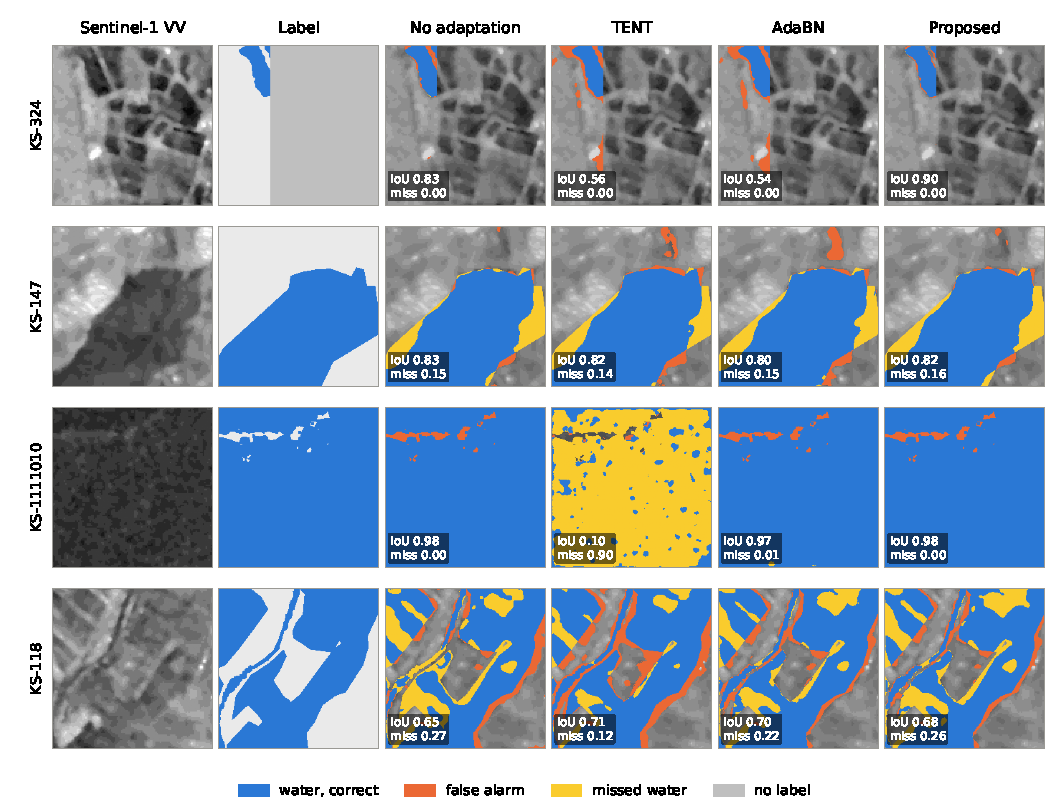
\includegraphics[width=\textwidth]{figures/fig_maps.pdf}
\caption{Example maps on Kuro Siwo (U-Net model seed 0, radar only) at the mean-rule threshold for the 20\% target, calibrated on the other events. Columns: Sentinel-1 VV (2$\times$2 averaged for display), label, and the maps of each method coloured by agreement with the label; IoU and miss rate refer to the shown chip. Grey label areas are unlabelled and not scored.}
\label{fig:maps}
\end{figure}

\subsection{Calibration without target labels}
\label{sec:transfer}
Same-dataset calibration needs labelled floods from the target dataset, which an emergency mapper may not have. Table~\ref{tab:transfer} and Fig.~\ref{fig:transfer} therefore repeat the comparison with thresholds calibrated once, on the 11 Sen1Floods11 floods, and applied unchanged. No Kuro Siwo or MMFlood label is used.

On Kuro Siwo the result depends entirely on adaptation. Without adaptation the source-calibrated threshold fails: the models miss 58\% of the water on average against a target of 20\%, and only 3 of 26 events meet the target. After any adaptation that re-estimates or trains the batch-norm layers, the target is met with a wide margin (mean miss rate 0.06--0.07). The proposed method is more accurate than the other two (IoU 0.557, against 0.426 for AdaBN and 0.346 for TENT; $+0.132$ over AdaBN, better on 25 of 26 events, Holm-corrected $p=10^{-6}$; $+0.211$ over TENT, 26 of 26, $p=3\times10^{-7}$) and the most even across floods: 25 of 26 events meet the target and the worst misses 23\% of its water, against 58--59\% for AdaBN and TENT. Because the realised miss rate is well below the target, the 30\% target is the more efficient operating point: there the proposed method reaches 0.672 IoU at a mean miss rate of 0.148 with 24 of 26 events below 30\%, which is the accuracy it reaches with same-dataset calibration. Physics-checked self-training without AdaBN reaches a higher IoU at the 20\% target (0.662), because its realised mean miss rate (0.156) sits closer to the target, but it is not reliable in this setting: only 20 of 26 events meet the target, one event misses 78\% of its water, and at the 30\% target the mean miss rate exceeds the target (0.321). The picture is the same with permanent water ignored: the source-calibrated threshold misses 62\% of the flood water without adaptation and 7\% with the proposed method (IoU 0.446 against 0.336 for AdaBN and 0.268 for TENT). EATA, SAR and CoTTA were not run on Sen1Floods11, so they have no source-calibrated threshold yet.

On MMFlood source-only calibration does not hold. At the 20\% target the realised mean miss rate is 0.28 without adaptation, 0.24 with AdaBN and 0.26 with the proposed method; only TENT stays below the target (0.19), at the lowest IoU. Calibrating on Sen1Floods11 and Kuro Siwo together (37 floods) does not help the adapted models either (mean miss rate 0.34--0.38). The Sen1Floods11 floods are evidently not exchangeable with the MMFlood activations, even after adaptation, for the reasons discussed in Section~\ref{sec:discussion}. Whether a source-calibrated threshold can be trusted on a new dataset therefore has to be checked, not assumed; on MMFlood the miss-rate statements of this paper hold only with same-dataset calibration.

\begin{table}[t]
\caption{Where the calibration floods come from: mean rule at the 20\% target, calibrated on the other floods of the same dataset or on the 11 Sen1Floods11 floods only (no label of the target dataset). Mean IoU, mean and worst per-flood miss rate, and floods meeting the target (mean over three models). Mean miss rates above the target are in italics.}
\label{tab:transfer}
\centering
\small
\setlength{\tabcolsep}{4pt}
\resizebox{\textwidth}{!}{\begin{tabular}{llcccccccc}
\toprule
 & & \multicolumn{4}{c}{Same-dataset calibration} & \multicolumn{4}{c}{Source-only calibration (Sen1Floods11)} \\
\cmidrule(lr){3-6}\cmidrule(lr){7-10}
Dataset & Method & IoU & Miss & Worst & Meeting & IoU & Miss & Worst & Meeting \\
\midrule
Kuro Siwo & No adaptation & 0.565 & 0.169 & 0.35 & 15.7/26 & 0.366 & \textit{0.583} & 0.95 & 2.7/26 \\
 & TENT & 0.468 & 0.176 & 0.92 & 19.7/26 & 0.346 & 0.073 & 0.59 & 23.3/26 \\
 & AdaBN & 0.562 & 0.171 & 0.88 & 17.7/26 & 0.425 & 0.072 & 0.58 & 23.7/26 \\
 & Physics check only & 0.666 & 0.171 & 0.85 & 19.0/26 & 0.662 & 0.156 & 0.78 & 19.7/26 \\
 & Proposed & 0.677 & 0.170 & 0.38 & 17.0/26 & 0.557 & 0.062 & 0.23 & 25.0/26 \\
\midrule
MMFlood & No adaptation & 0.110 & 0.176 & 0.72 & 21.0/30 & 0.150 & \textit{0.280} & 0.82 & 16.3/30 \\
 & TENT & 0.096 & 0.172 & 0.57 & 19.7/30 & 0.103 & 0.186 & 0.61 & 18.7/30 \\
 & AdaBN & 0.098 & 0.177 & 0.65 & 20.0/30 & 0.128 & \textit{0.242} & 0.74 & 17.3/30 \\
 & Proposed & 0.112 & 0.177 & 0.78 & 19.7/30 & 0.157 & \textit{0.256} & 0.90 & 17.0/30 \\
\bottomrule
\end{tabular}
}
\end{table}

\begin{figure}[t]
\centering
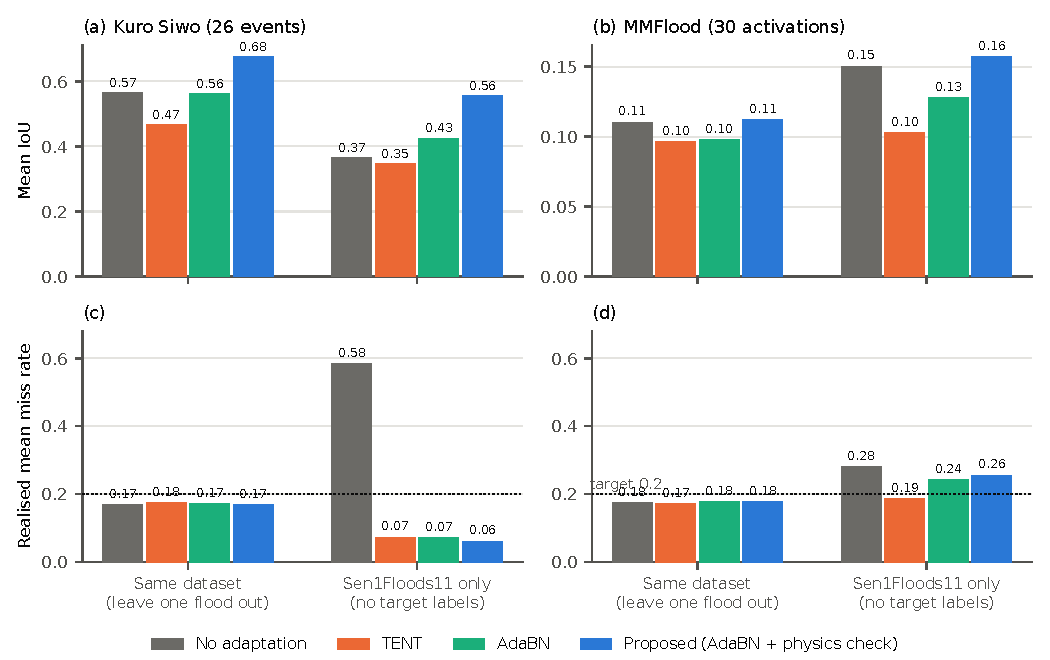
\includegraphics[width=\textwidth]{figures/fig_transfer.pdf}
\caption{Mean IoU (a, b) and realised mean miss rate (c, d) under the mean rule at the 20\% target, with same-dataset calibration and with calibration on Sen1Floods11 only. On Kuro Siwo the source-calibrated threshold fails without adaptation and holds after it; on MMFlood it fails for three of the four methods.}
\label{fig:transfer}
\end{figure}

\subsection{Per-flood rule}
\label{sec:perflood}
The mean rule leaves a third of the floods above the target. The per-flood rule (Eq.~\ref{eq:flood}) trades accuracy for coverage (Table~\ref{tab:perflood}). With same-dataset calibration and $\delta=0.2$, between 80\% and 83\% of the floods miss at most 20\% of their water on all three datasets and for every method, as the rule promises; with $\delta=0.1$ the share is 90--92\%. On Kuro Siwo the proposed method keeps an IoU of 0.652 under this stricter rule, close to its 0.677 under the mean rule, whereas no adaptation, AdaBN and TENT fall to 0.529, 0.535 and 0.413, and EATA, SAR and CoTTA to 0.517--0.554 (the proposed method is better than each of the six on at least 24 of 26 events, Holm-corrected $p\le5\times10^{-6}$). It remains level with the fine-tuned models (0.643). On MMFlood all methods are within 0.011 IoU of each other. Floods above the target remain, by construction, in up to a share $\delta$ of cases, and their miss rates can be high.

\begin{table}[t]
\caption{Per-flood rule at $\alpha=0.2$ with same-dataset calibration: mean IoU, number (share) of floods that miss at most 20\% of their water, and the worst per-flood miss rate. Mean over three models for Kuro Siwo and MMFlood.}
\label{tab:perflood}
\centering
\small
\resizebox{\textwidth}{!}{\begin{tabular}{llcccccc}
\toprule
 & & \multicolumn{3}{c}{$\delta=0.2$ (at least 80\% of floods)} & \multicolumn{3}{c}{$\delta=0.1$ (at least 90\% of floods)} \\
\cmidrule(lr){3-5}\cmidrule(lr){6-8}
Dataset & Method & IoU & Meeting & Worst & IoU & Meeting & Worst \\
\midrule
Sen1Floods11 & No adaptation & \textbf{0.475} & 9.0/11 (82\%) & 0.26 & \textbf{0.447} & 10.0/11 (91\%) & 0.24 \\
 & TENT & 0.405 & 9.0/11 (82\%) & 0.48 & 0.345 & 10.0/11 (91\%) & 0.25 \\
 & AdaBN & 0.459 & 9.0/11 (82\%) & 0.27 & 0.402 & 10.0/11 (91\%) & 0.26 \\
 & Proposed & 0.459 & 9.0/11 (82\%) & 0.34 & 0.360 & 10.0/11 (91\%) & 0.26 \\
\midrule
Kuro Siwo & No adaptation & 0.529 & 21.7/26 (83\%) & 0.23 & 0.500 & 24.0/26 (92\%) & 0.21 \\
 & TENT & 0.413 & 21.3/26 (82\%) & 0.84 & 0.287 & 24.0/26 (92\%) & 0.45 \\
 & AdaBN & 0.535 & 21.0/26 (81\%) & 0.83 & 0.315 & 24.0/26 (92\%) & 0.61 \\
 & Proposed & \textbf{0.652} & 21.0/26 (81\%) & 0.28 & \textbf{0.615} & 24.0/26 (92\%) & 0.26 \\
\midrule
MMFlood & No adaptation & 0.082 & 24.0/30 (80\%) & 0.65 & 0.061 & 27.0/30 (90\%) & 0.48 \\
 & TENT & 0.077 & 24.3/30 (81\%) & 0.39 & 0.068 & 27.3/30 (91\%) & 0.36 \\
 & AdaBN & 0.072 & 25.0/30 (83\%) & 0.39 & 0.063 & 27.3/30 (91\%) & 0.27 \\
 & Proposed & \textbf{0.083} & 24.7/30 (82\%) & 0.36 & \textbf{0.074} & 27.0/30 (90\%) & 0.29 \\
\bottomrule
\end{tabular}
}
\end{table}

\subsection{MMFlood: pre-registered final test}
\label{sec:mm}
Table~\ref{tab:mm} reports the primary analysis on 30 activations with same-dataset calibration. Of the four pre-registered hypotheses, three are supported and one is not. H1 and H2 are supported: under the mean rule at the 20\% target the proposed method beats TENT by 0.016 IoU (better on 28 of 30 activations, Holm-corrected $p=4\times10^{-8}$) and AdaBN by 0.014 (28 of 30, $p=6\times10^{-8}$). H3 is not supported: at threshold 0.5 the mean gain over no adaptation is 0.011, but the method is better on only 11 of 30 activations ($p=0.87$); a few large gains (e.g.\ Slovenia, 0.06 to 0.54) raise the mean while most activations are slightly worse. H4 is supported: the mean miss rate at the 20\% target is 0.177. The analysis with region folders as units gives the same verdicts.

These verdicts need three qualifications. First, the proposed method is not better than no adaptation at a matched miss rate either (0.112 against 0.110 IoU; better on 16 of 30 activations, $p=0.76$, post hoc): on MMFlood adaptation with the physics check does no harm and brings no gain. Second, the differences behind H1 and H2 are consistent across activations but small in absolute terms, and at an IoU of about 0.11 no method yields a usable map at this target. Third, plain adaptation tends to lower the accuracy of calibrated maps: AdaBN is worse than no adaptation by 0.012 IoU (no adaptation better on 22 of 30 activations, Holm-corrected $p=0.024$, post hoc), and TENT by 0.014, which is not significant (17 of 30, $p=0.11$). Absolute accuracy is low for every method and varies strongly between activations, from 0.01 (Uganda, EMSR438) to 0.54 (Slovenia, EMSR107) at 0.5; Section~\ref{sec:discussion} examines why.

\begin{table}[t]
\caption{MMFlood, pre-registered test, 30 activations (U-Net, three models), same-dataset calibration: mean IoU at threshold 0.5, under the mean rule and under the per-flood rule, with the number of activations that meet the 20\% target under the per-flood rule. Under the mean rule at the 20\% target the realised mean miss rate is 0.172--0.177 for every method.}
\label{tab:mm}
\centering
\small
\begin{tabular}{lcccccc}
\toprule
 & & \multicolumn{3}{c}{Mean rule, target $\alpha$} & \multicolumn{2}{c}{Per-flood rule, $\alpha=\delta=0.2$} \\
\cmidrule(lr){3-5}\cmidrule(lr){6-7}
Method & 0.5 & 10\% & 20\% & 30\% & IoU & Floods meeting \\
\midrule
No adaptation & 0.193 & 0.068 & 0.110 & 0.146 & 0.082 & 24.0/30 \\
TENT-R (running statistics) & 0.192 & 0.071 & 0.096 & 0.127 & 0.077 & 24.3/30 \\
AdaBN & 0.195 & 0.064 & 0.098 & 0.140 & 0.072 & 25.0/30 \\
AdaBN + physics check, fixed rule & \textbf{0.211} & \textbf{0.079} & 0.112 & 0.158 & \textbf{0.085} & 25.0/30 \\
AdaBN + physics check, adaptive rule (proposed) & 0.203 & 0.077 & \textbf{0.112} & \textbf{0.165} & 0.083 & 24.7/30 \\
\midrule
Otsu threshold on VV (no model) & 0.090 & -- & -- & -- & -- & -- \\
\bottomrule
\end{tabular}

\end{table}

\subsection{Second backbone}
With the pretrained ResNet-34 U-Net (exploratory), the unadapted model collapses on Kuro Siwo, predicting almost no water at 0.5 (IoU 0.035). The proposed method recovers an IoU of 0.627 at 0.5 and 0.628 under the mean rule at the 20\% target, against 0.541 for AdaBN, 0.276 for TENT and 0.229 without adaptation, and beats TENT and no adaptation on all 26 events and AdaBN on 19 (Table~\ref{tab:r34}). On MMFlood the same pattern appears as with the U-Net: at the 20\% target the proposed method beats TENT on 30 of 30 activations (Holm-corrected $p=3\times10^{-9}$) and AdaBN on 28 of 30 ($p=4\times10^{-6}$), and at 0.5 it does not beat the unadapted model (11 of 30). TENT is clearly harmful with this backbone (0.053 against 0.109 without adaptation at the 20\% target). Adding 33 Kuro Siwo floods to training did not raise MMFlood accuracy (0.207 at 0.5 without adaptation), and the proposed method again beat AdaBN at the 20\% target (27 of 30, $p=10^{-4}$). With the ResNet-34 models the proposed method is not harmless at the default threshold, however: at 0.5 its IoU on MMFlood is below that of the unadapted model (0.188 against 0.192, and 0.182 against 0.207 for the model trained with Kuro Siwo), because it maps more water and the additional water is often wrong on this dataset. Only at a matched miss rate is it at or above the unadapted model in all three cases. The realised mean miss rate at the 20\% target was at or below 0.18 for every model and method.

\begin{table}[t]
\caption{Second backbone and more diverse training data (exploratory): mean IoU at 0.5 / under the mean rule at the 20\% target (same-dataset calibration); MMFlood uses activations as units. ``+KS'' denotes training on Sen1Floods11 plus 1,962 Kuro Siwo chips (33 events); Kuro Siwo is then no longer a test set for that model.}
\label{tab:r34}
\centering
\begin{tabular}{lcccc}
\toprule
 & Kuro Siwo (26) & \multicolumn{3}{c}{MMFlood (30 activations)} \\
\cmidrule(lr){2-2}\cmidrule(lr){3-5}
Method & ResNet-34 & U-Net & ResNet-34 & ResNet-34 +KS \\
\midrule
No adaptation & 0.035 / 0.229 & 0.193 / 0.110 & 0.192 / 0.109 & 0.207 / 0.117 \\
TENT & 0.454 / 0.276 & 0.192 / 0.096 & 0.158 / 0.053 & -- \\
AdaBN & 0.560 / 0.541 & 0.195 / 0.098 & 0.198 / 0.104 & 0.204 / 0.106 \\
Proposed & 0.627 / 0.628 & 0.203 / 0.112 & 0.188 / 0.122 & 0.182 / 0.121 \\
\bottomrule
\end{tabular}
\end{table}

\subsection{Sensitivity to the settings}
Table~\ref{tab:sens} changes one setting of the proposed method at a time on Kuro Siwo (model seed 0; for this model AdaBN, TENT and no adaptation reach 0.560, 0.530 and 0.586 IoU at the 20\% target). At the 20\% target every variant stays between 0.638 and 0.671 IoU, against 0.665 with the defaults, and the mean miss rate stays at 0.170--0.172. The HAND limit hardly matters (3 or 10\,m instead of 5\,m change IoU by at most 0.001), presumably because pixels that pass the darkness and slope tests rarely lie more than a few metres above the drainage network. Moving the dark-threshold caps by 2\,dB or the confidence thresholds to 0.8/0.2 or 0.95/0.05 costs at most 0.011. Fewer self-training steps cost the most (100 steps: $-0.027$), and 400 steps help slightly ($+0.006$). The results therefore do not hinge on a finely tuned setting.

\begin{table}[t]
\caption{Sensitivity of the proposed method (AdaBN + adaptive physics-checked self-training) on Kuro Siwo, U-Net model seed 0, one setting changed at a time from the defaults (caps $-15/-22$\,dB, HAND limit 5\,m, 200 steps, confidence 0.9/0.1): mean IoU at 0.5 and under the mean rule (same-dataset calibration), mean miss rate and events meeting the target at the 20\% target.}
\label{tab:sens}
\centering
\begin{tabular}{lcccccc}
\toprule
Setting & 0.5 & 10\% & 20\% & 30\% & Miss rate & Meeting 20\% \\
\midrule
Defaults & 0.654 & 0.561 & 0.665 & 0.625 & 0.170 & 16/26 \\
Caps $-17/-24$\,dB & 0.655 & 0.543 & 0.659 & 0.625 & 0.170 & 17/26 \\
Caps $-13/-20$\,dB & 0.640 & 0.576 & 0.655 & 0.616 & 0.170 & 16/26 \\
HAND limit 3\,m & 0.655 & 0.561 & 0.665 & 0.626 & 0.170 & 16/26 \\
HAND limit 10\,m & 0.654 & 0.560 & 0.664 & 0.625 & 0.170 & 16/26 \\
100 steps & 0.628 & 0.541 & 0.638 & 0.622 & 0.172 & 15/26 \\
400 steps & 0.671 & 0.571 & 0.671 & 0.628 & 0.170 & 15/26 \\
Confidence 0.8/0.2 & 0.651 & 0.567 & 0.655 & 0.619 & 0.170 & 17/26 \\
Confidence 0.95/0.05 & 0.637 & 0.553 & 0.654 & 0.619 & 0.170 & 15/26 \\
\bottomrule
\end{tabular}
\end{table}

%% =====================================================================
\section{Discussion}
\label{sec:discussion}

\paragraph{What calibration gives, and what it does not.} With calibration floods from the same dataset, the mean rule kept the mean miss rate at or just below the target on all three datasets, including MMFlood, which played no part in any design decision, and the per-flood rule delivered the promised share of floods. Three caveats define the scope of these statements. They are statements about floods in general: under the mean rule about a third of the floods missed more than the target (the worst MMFlood activation 78\%), and under the per-flood rule a share $\delta$ still does. They need labelled floods that resemble the one being mapped; on Kuro Siwo, most of the gain of the unadapted model from 0.186 to 0.565 IoU comes from such labels and not from adaptation. And they do not carry over to a new dataset on their own: a threshold calibrated on Sen1Floods11 missed 58\% of the water on Kuro Siwo without adaptation, and 24--28\% on MMFlood for three of four methods.

\paragraph{Adaptation and calibration interact.} The same experiment shows what adaptation is good for. On Kuro Siwo every method that re-estimates or trains the batch-norm layers brought the source-calibrated threshold back below the target, because the shift between the two datasets is largely a shift in radiometry and land cover that batch-norm statistics absorb; the model's scores then mean roughly the same on both datasets. The physics check adds accuracy on top (0.557 against 0.425 IoU for AdaBN alone) and evens out the floods, with 25 of 26 events below the target. In the other direction, calibration changes the verdict on adaptation. At threshold 0.5 on Kuro Siwo, TENT, EATA, SAR, CoTTA and AdaBN each appear to gain about 0.4 IoU over the unadapted model; at a matched miss rate none of them gains anything, and TENT loses 0.10, plausibly because entropy minimisation sharpens the scores of each flood separately and makes them less comparable across floods. The safeguards that EATA, SAR and CoTTA add to entropy minimisation and self-training protect against collapse but do not add information about where the water is; the physics check does, and it is the only adaptation here whose gain survives calibration, to the level of supervised fine-tuning on labelled floods of the target dataset. Comparing adaptation methods at a fixed threshold therefore mixes up accuracy and operating point.

\paragraph{When adaptation does not help.} On MMFlood no adaptation method improved on the unadapted model at a matched miss rate. AdaBN alone was significantly worse, TENT worse on average, and the proposed method level. At the default threshold the proposed method raised mean IoU slightly for the U-Net but lowered it for both ResNet-34 models. The physics check thus limits the damage that adaptation can do when the model's errors are not the kind that dark, low-lying pixels can correct, but it is no guarantee of improvement, and we do not claim that it makes adaptation safe.

\paragraph{Low accuracy on MMFlood.} All methods reach only about 0.2 IoU on MMFlood at 0.5. The Sen1Floods11 models transfer poorly to MMFlood's 20\,m images (upsampled to 10\,m), to its labels drawn from EMS rapid-mapping polygons, and to its many floods under vegetation or in built-up areas, where water is not dark \citep{tsyganskaya2018vegetation,zhao2024urbansarfloods}. Lowering the threshold to meet a miss-rate target then brings many false alarms. Neither a pretrained ResNet-34 backbone nor 33 additional training floods from Kuro Siwo raised MMFlood accuracy (0.19--0.21 IoU at 0.5 for all three models), which suggests that the ceiling is set by the mismatch between MMFlood's images and labels and our single-date radar input rather than by model capacity.

A second reason is the small share of flood water. The median MMFlood activation has 2.5\% of its valid pixels labelled as flood water, against 10.4\% for a Kuro Siwo event and 11.8\% for a Sen1Floods11 event (Fig.~\ref{fig:mmwater}a). With so little water, a false-alarm rate of only 2.5\% of dry pixels already produces about as many false water pixels as there are true ones, and IoU falls accordingly. Across the 30 activations, IoU rises with the water share (Spearman $\rho=0.62$, $p=2\times10^{-4}$; Fig.~\ref{fig:mmwater}b): the 12 activations with less than 2\% water average 0.10 IoU, the 5 with at least 5\% average 0.35. Published MMFlood baselines \citep{montello2022mmflood} report the mean IoU over the flood and background classes for models trained on MMFlood itself, which the dominant background class inflates, so they are not directly comparable to our water-class IoU after a dataset shift. A model-free reference confirms that MMFlood is hard rather than mishandled: an Otsu threshold on VV, fitted per region folder, reaches only 0.090 IoU on average over the 30 activations (median 0.063), less than half of what every network achieves, whereas on Kuro Siwo the same threshold reaches 0.456. The Otsu IoU also follows the water share, from 0.010 in Germany (EMSR261, 0.5\% water) to 0.30 in Finland--Sweden, Albania and Guyana (6--11\% water). We also checked the raw MMFlood files for eight region folders (Table~\ref{tab:mmraw}). The stored backscatter is linear power (median VV between $-12.7$ and $-7.3$\,dB after conversion), the masks contain only 0 and 1, and the same Otsu threshold gives a similar IoU on our resampled 10\,m chips as on the native 20\,m grid (within 0.03 in six folders, higher on the chips in the other two, whose chips contain more of the flooded area), so neither the unit conversion nor the resampling misaligns images and labels. What the check does reveal is that much of the labelled water is not dark: in the median folder only 40\% of labelled water pixels lie below $-15$\,dB in VV, and in Uganda (EMSR438) labelled water is brighter than dry land (median $-5.8$ against $-9.3$\,dB), as expected for flooded vegetation or built-up areas. Such water is invisible to any method that relies on single-date backscatter, including our physics check.

\begin{table}[t]
\caption{MMFlood raw-data check on one image of eight region folders: labelled water share, median VV backscatter of labelled water and of dry land, share of labelled water darker than $-15$\,dB, and IoU of a per-image Otsu threshold on the native 20\,m grid and, with the same threshold, on our 10\,m chips. Backscatter in dB; country codes ISO 3166.}
\label{tab:mmraw}
\centering
\begin{tabular}{lcccccc}
\toprule
Folder & Water & VV water & VV dry & Water $<-15$\,dB & Otsu, 20\,m & Otsu, chips \\
\midrule
EMSR107-5 (SI) & 3.6\% & $-15.7$ & $-8.7$ & 56\% & 0.077 & 0.080 \\
EMSR167-2 (BE) & 1.1\% & $-12.9$ & $-8.8$ & 30\% & 0.021 & 0.006 \\
EMSR184-4 (AU) & 19.8\% & $-19.7$ & $-10.2$ & 78\% & 0.465 & 0.579 \\
EMSR203-3 (US) & 5.8\% & $-13.3$ & $-10.5$ & 35\% & 0.093 & 0.116 \\
EMSR265-14 (FR) & 24.4\% & $-20.0$ & $-9.2$ & 93\% & 0.744 & 0.770 \\
EMSR438-5 (UG) & 2.2\% & $-5.8$ & $-9.3$ & 2\% & 0.002 & 0.001 \\
EMSR479-0 (MX) & 0.3\% & $-10.1$ & $-7.3$ & 13\% & 0.006 & 0.010 \\
EMSR514-0 (GY) & 12.3\% & $-14.4$ & $-12.2$ & 46\% & 0.132 & 0.366 \\
\bottomrule
\end{tabular}
\end{table}

\begin{figure}[t]
\centering
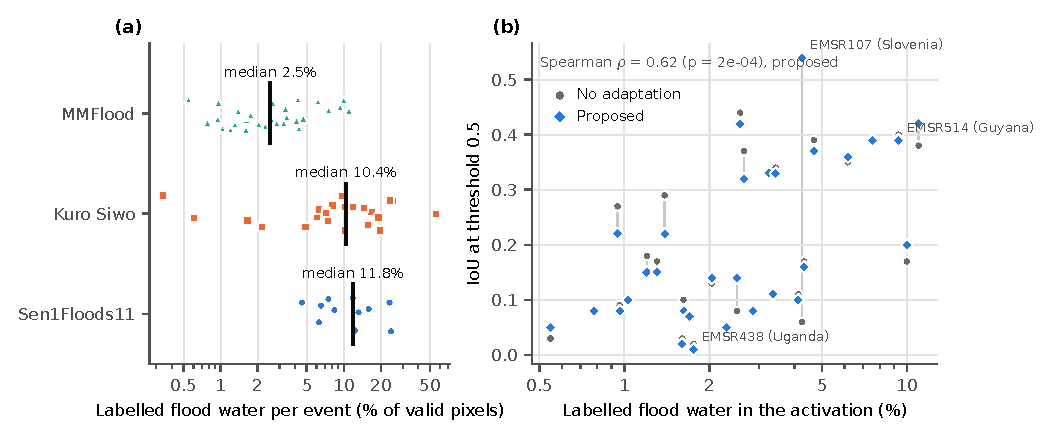
\includegraphics[width=\textwidth]{figures/fig_mmflood_water.pdf}
\caption{(a) Share of valid pixels labelled as flood water, per Sen1Floods11 event, Kuro Siwo event and MMFlood activation (log scale; bar: median). (b) MMFlood: IoU at threshold 0.5 per activation against its water share, without adaptation and with the proposed method (mean over three models).}
\label{fig:mmwater}
\end{figure}

\paragraph{Base models.} The models are small and trained on 252 chips; they are baselines, not the state of the art. We did not evaluate a geospatial foundation model. The adaptation studied here acts on batch-normalisation layers, which the transformer encoders of current foundation models such as Prithvi \citep{jakubik2023prithvi} do not have, so the method would not apply to them unchanged; whether the calibration findings carry over to such models is open. The ResNet-34 experiments indicate that the pattern does not depend on the specific convolutional backbone, and that neither ImageNet pretraining nor 33 additional training floods lifted the MMFlood ceiling.

\paragraph{Limitations.} (i) Both calibration rules need labelled floods exchangeable with the new one; with source-only calibration the target was met on Kuro Siwo after adaptation but not on MMFlood, and we know of no label-free test that tells the two cases apart in advance \citep{tibshirani2019covshift,barber2023beyond}. (ii) The per-flood rule covers a share $1-\delta$ of floods; stricter per-flood control \citep{bates2021rcps} needs more calibration events than the 11 to 30 available here. (iii) The dark-water rule cannot detect flooded vegetation or urban flooding. (iv) The adaptive rule and the combination with AdaBN were chosen on Kuro Siwo, so only MMFlood is an untouched test of them, and on MMFlood the gains are small. (v) Results use three seeds and a sample of Kuro Siwo that covers 33 of its 43 events at about one patch in 50. (vi) With $n$ calibration floods, targets below $1/(n+1)$ are unattainable except by mapping everything as water, so strict targets need many calibration floods. (vii) The sensitivity analysis used one model; the settings were robust there, but their interaction was not explored. (viii) The pre-registration was not deposited in a public registry before the test. (ix) Sen1Floods11 and Kuro Siwo label permanent water as water while MMFlood ignores it, which adds a label shift to the comparison between datasets; ignoring permanent water on Kuro Siwo lowered every score by about 0.10 IoU without changing the order of the methods. (x) All analyses other than the four MMFlood hypotheses are post hoc. (xi) EATA, SAR, CoTTA and the supervised reference were run on Kuro Siwo only. (xii) On Kuro Siwo flood water, a per-event dark threshold without any model comes within 0.04 IoU of the proposed method at threshold 0.5, so part of what the method achieves there is to pass the darkness cue to the network.

%% =====================================================================
\section{Conclusion}
\label{sec:conclusion}
We proposed a label-free test-time adaptation for SAR flood mapping that checks pseudo-labels against radar and terrain physics, and evaluated it together with a calibration of the map threshold across flood events, at matched miss rates, on three datasets. With calibration floods from the same dataset the mean miss rate stayed at the chosen target everywhere, and a per-flood rule kept four floods in five below it. Where the radar shift is large (Kuro Siwo) the method was more accurate than six adaptation baselines at every matched miss rate, none of which improved on the unadapted model there, and level with supervised fine-tuning; it also turned a threshold calibrated on the source dataset alone from badly invalid into valid, for which no target label was needed. On the pre-registered MMFlood test it beat TENT and AdaBN at a matched miss rate but not the unadapted model, source-only calibration failed, and accuracy was too low for use, largely because much of the labelled water there is not dark. Future work should test the approach with stronger, foundation-model backbones and normalisation-free adaptation, bring in the pre-flood image, extend the physics check to flooded vegetation and urban areas, and look for label-free indicators of when a source-calibrated threshold can be trusted.

%% =====================================================================
\section*{Declaration of competing interest}
The authors declare that they have no known competing financial interests or personal relationships that could have appeared to influence the work reported in this paper.

\section*{Funding}
This research did not receive any specific grant from funding agencies in the public, commercial, or not-for-profit sectors.

\section*{Data availability}
All datasets used are publicly available: Sen1Floods11 \citep{bonafilia2020sen1floods11}, Kuro Siwo \citep{bountos2024kurosiwo}, MMFlood \citep{montello2022mmflood} and the GLO-30 HAND tiles \citep{glo30hand2022}. The code, the MMFlood exclusion list, the pre-registration text and the stored results behind every table and figure are available at \url{https://github.com/Mahim25800/Research-Flood}.

\section*{Declaration of generative AI and AI-assisted technologies in the manuscript preparation process}
During the preparation of this work the authors used Claude (Anthropic) to assist with code development, running and monitoring the experiments, literature search, preparing figures, drafting and language editing, and formatting the manuscript to the journal template. After using this tool, the authors reviewed and edited the content as needed and take full responsibility for the content of the published article.

\section*{Acknowledgements}
The authors thank the Department of Computer Science, American International University-Bangladesh, for its support.

\section*{CRediT authorship contribution statement}
\textbf{MD Sakib Hasan:} Conceptualization, Data curation, Investigation, Methodology, Resources, Writing -- original draft, Writing -- review \& editing. \textbf{Mostofa Seum:} Conceptualization, Data curation, Investigation, Methodology, Writing -- original draft, Writing -- review \& editing. \textbf{Meer Mursalin:} Data curation, Investigation, Methodology, Visualization, Writing -- review \& editing. \textbf{Tanvir Ahmed:} Project administration, Supervision, Validation, Writing -- review \& editing. \textbf{Rifath Mahmud:} Project administration, Supervision, Validation, Writing -- review \& editing. \textbf{Syeda Anika Tasnim:} Project administration, Supervision, Validation, Writing -- review \& editing.

\bibliographystyle{unsrtnat}
\bibliography{references}

\end{document}
